% Números e fontes: proposta/evidencias.csv e tabela do README.md deste diretório.
% Detalhes técnicos, decisões e pendências: proposta/pendencias.md.
\documentclass[11pt,a4paper]{article}

\usepackage{fontspec}
\usepackage[brazilian]{babel}
\usepackage[margin=2.5cm]{geometry}
\usepackage{microtype}
\usepackage{icomma}
\usepackage{booktabs,tabularx,float,array,makecell}
\usepackage{enumitem}
\usepackage{graphicx}
\usepackage[hidelinks]{hyperref}

\setlist{itemsep=2pt,topsep=4pt}
\setlength{\emergencystretch}{3em}
\newcolumntype{Y}{>{\raggedright\arraybackslash}X}

\title{Quantificação da incerteza na estimativa da área de garimpo em imagens de satélite}
\author{Emanuel Pires\\[2pt] \small Proposta de dissertação de mestrado}
\date{3 de novembro de 2026}

\begin{document}
\maketitle

\section{Introdução}

O mapeamento de áreas de mineração por satélite já foi feito em escala regional e global
\cite{couttenier2022,tang2023,jasansky2025}. O LIGEM.Redes (Laboratório Integrado de Geointeligência e Modelagem de
Redes de Ilícitos da Amazônia) inclui em seu plano de trabalho a criação de um método semiautomatizado para estimar áreas de mineração com imagens de satélite e aprendizado de máquina \cite{ligemprojetos}.

Uma área em hectares, por si só, não informa quanto pode estar errada. Em um mapa, ela é calculada somando pixels, então pequenos erros nas bordas se acumulam no resultado. Há indícios de que isso pesa na mineração. Na
validação de um mapa global, metade dos pontos com divergência estava a menos de 50\,m das bordas dos polígonos, contra
16\% dos pontos concordantes \cite{maus2020}. No Amazon Mining Watch, os autores relatam que a área segmentada fica em
cerca de 1,5 vez a extensão anotada manualmente, em 184 amostras de avaliação \cite{amw2026}.

Uma alternativa é apresentar a área como um intervalo, por exemplo, entre 10 e 14\,ha, em vez de um único valor. A
predição conformal permite construir esses intervalos a partir de erros observados, com a garantia de que contêm o valor
de referência em uma proporção escolhida dos casos, desde que os dados novos sejam comparáveis aos usados na calibração
\cite{lei2018}. Essa condição é o ponto crítico em sensoriamento remoto, porque um intervalo calibrado em um continente
pode não funcionar em outro \cite{tibshirani2019,barber2023}. Intervalos de área calibrados em uma região continuam
confiáveis em outra?

\section{Objetivos}

O objetivo geral é investigar, de forma exploratória, se é possível acompanhar a área de garimpo estimada por
modelos de segmentação com intervalos confiáveis e úteis em regiões não vistas no treinamento. Os objetivos
específicos são:

\begin{enumerate}[leftmargin=*]
  \item analisar como o erro de área se relaciona com a qualidade da segmentação e das bordas;
  \item comparar métodos de construção de intervalos quanto à confiabilidade e à largura;
  \item medir o quanto a confiabilidade muda quando a calibração é feita em outro continente.
\end{enumerate}

\section{Trabalhos relacionados}

\textbf{Mapeamento de mineração.} Há mapeamentos globais \cite{tang2023} e tropicais \cite{jasansky2025}. Para mineração
artesanal, \cite{couttenier2022} mapearam minas em 13 países da África Ocidental, sem relatar intervalos para a área. Na
Amazônia, destacam-se o Amazon Mining Watch \cite{amw2026} e o estudo local de \cite{silva2025}, em Mato Grosso. Com
imagens de drone no Peru, \cite{cui2026} criaram uma base de comparação para segmentação, sem tratar de incerteza. O
trabalho mais próximo que encontramos em garimpo é o de \cite{okumura2026}, que propõe um índice de atividade com medida de confiança,
mas acompanha a direção da mudança, e não a área.

\textbf{Incerteza em observação da Terra.} \cite{singh2024} aplicam predição conformal a produtos de observação da
Terra, com foco em predições individuais. \cite{lehmann2026} analisam a calibração de modelos sob imagens
degradadas artificialmente, e \cite{gonzalez2026} usam a incerteza para decidir quando o modelo deve se abster.

\textbf{Predição conformal em segmentação.} Parte dos trabalhos indica quais pixels podem pertencer ao objeto
\cite{mossina2024,viti2026}, o que não fornece um intervalo em hectares. O método mais próximo desta proposta que encontramos é o
COMPASS \cite{cheung2026}, que gera intervalos de área e, em quatro conjuntos de imagens médicas, obteve intervalos
cerca de 10\% a 35\% mais estreitos que os da abordagem conformal simples. Ele será um dos métodos comparados, adaptado para imagens de satélite.

\textbf{Estimativa de área por amostragem.} Métodos como os de \cite{olofsson2014} e a inferência potencializada por
predição \cite{angelopoulos2023,lu2025} usam uma amostra de referência para produzir estimativas sobre uma população
inteira. Esta proposta faz outra pergunta: quanto há em um local específico já identificado, sem nova amostra local.

A contribuição pretendida é comparar, em imagens de satélite, métodos de intervalo de área, incluindo o COMPASS, avaliado por
seus autores em imagens médicas, em um problema em que a mudança de região
faz parte do uso real.

\section{Questões de pesquisa}

O estudo é exploratório e responderá às seguintes questões:

\begin{enumerate}[leftmargin=*,label=Q\arabic*.]
  \item \textbf{Como o erro de área se relaciona com a qualidade da segmentação nas bordas?} Para cada célula de imagem com
  mineração, serão calculados o erro de área, em hectares e em percentual da área de referência, e a qualidade da segmentação,
  pelo coeficiente Dice e pelo F1 de fronteira. A correlação de Spearman entre essas medidas, por modelo, indicará quanto o erro
  de área acompanha a qualidade das bordas. O viés, isto é, o erro médio com sinal, indicará se os modelos tendem a superestimar
  ou subestimar a área.
  \item \textbf{Qual método se ajusta melhor à estimativa da área de garimpo, mantendo a cobertura com a menor largura?} A
  cobertura é a proporção de casos em que a área de referência cai dentro do intervalo, com meta de 90\%. Para cada método e
  modelo, serão calculadas a cobertura e a largura média no teste, com calibração em outros continentes. Serão considerados
  ajustados os métodos cujo intervalo de 95\% da cobertura incluir a meta; entre eles, o melhor será o de menor largura. O
  \emph{interval score} \cite{gneiting2007}, que soma à largura uma penalidade quando a referência fica fora do intervalo,
  resumirá os dois critérios em um único número.
  \item \textbf{Quanto a confiabilidade cai quando a calibração vem de outro continente?} Cada método será calibrado nas
  situações da Tabela~\ref{tab:combinacoes} e testado nas mesmas células. A diferença de cobertura e de largura entre a calibração
  em outros continentes e a calibração na própria região medirá a queda, e a diferença em relação à calibração ponderada mostrará
  quanto a ponderação recupera.
\end{enumerate}

\section{Metodologia}

\textbf{Dados.} A base será um conjunto público de máscaras de mineração verificadas manualmente, associado a imagens
Sentinel-2 de 10\,m \cite{jasansky2024}. Ele reúne 1.207 recortes de imagem com divisão definida, dos quais 232 são de
mineração artesanal e 54 estão na Amazônia brasileira. Cada recorte será dividido em células de tamanho fixo. Recortes a
menos de 50\,km entre si formarão um mesmo grupo, e a análise tratará cada grupo como uma unidade \cite{dunn2022}. Isso
resulta em 75 grupos artesanais, 12 deles na Amazônia brasileira. A Figura~\ref{fig:exemplos} mostra exemplos, com a área
da máscara e o ano da imagem.

\begin{figure}[H]
\centering
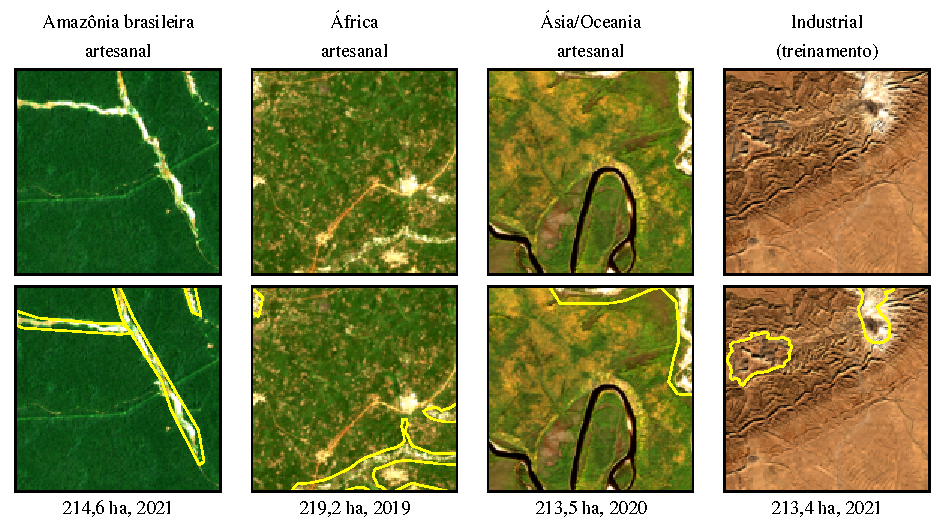
\includegraphics[width=\linewidth]{exemplos_dataset.pdf}
\caption{Células de $512 \times 512$ pixels do conjunto de dados, em cor natural, sem (acima) e com (abaixo) a máscara de referência, em amarelo.}
\label{fig:exemplos}

\small Fonte: elaboração própria, com máscaras de \cite{jasansky2024} e dados Copernicus Sentinel modificados.
\end{figure}

\textbf{Divisão dos dados.} O treinamento e a calibração usarão regiões da Ásia, Oceania, África e Europa. O teste usará
24 grupos das Américas, incluindo a Amazônia, e nenhum exemplo artesanal das Américas será usado no treinamento. Assim, o
teste simula a aplicação do modelo em uma região nova.

\textbf{Referência.} As máscaras preferidas do conjunto de dados serão a referência de área, sem nova anotação. Seus autores
revalidaram manualmente os recortes de teste e estimaram precisão de 99,22\% e revocação de 95,71\% \cite{jasansky2024}.

\textbf{Modelos.} Serão comparados dois tipos de modelo de segmentação: uma rede convolucional simples (ConvNet), sem
conexões de salto, e a U-Net \cite{unet}, cada um treinado uma única vez. As duas arquiteturas permitem verificar se o comportamento dos métodos de intervalo depende do modelo.

\textbf{Intervalos.} Depois do treinamento, os intervalos serão calculados por sete métodos: um cálculo sem calibração, que serve de controle, a predição conformal simples, método clássico usado como base de comparação \cite{lei2018}, três variações dela e duas versões adaptadas do COMPASS \cite{cheung2026}. O COMPASS será adaptado ao uso de imagens de
satélite, à área em hectares e ao teste entre continentes, tendo como referência o código público dos autores
\cite{compasscode}. A calibração será
comparada em três situações: com dados de outros continentes, com esses mesmos dados ponderados para se aproximarem da
região de teste \cite{tibshirani2019} e com dados da própria região de teste. A Tabela~\ref{tab:combinacoes} apresenta as
combinações, aplicadas aos dois modelos.

\begin{table}[H]
\centering\small
\caption{Combinações de métodos de intervalo e situações de calibração a comparar.}
\label{tab:combinacoes}
\begin{tabularx}{\linewidth}{>{\raggedright\arraybackslash}p{4.4cm}Yccc}
\toprule
& & \multicolumn{3}{c}{Calibração} \\
\cmidrule(lr){3-5}
Método & Como gera o intervalo & \makecell{Outro\\continente} & \makecell{Outro continente,\\ponderada} & \makecell{Própria\\região} \\
\midrule
Sem calibração & Soma a incerteza dos pixels, tratados como independentes; serve de controle & --- & --- & --- \\
Conformal simples & Margem fixa em hectares, igual para todas as células & Sim & Sim & Sim \\
Conformal relativo & Margem proporcional à área estimada & Sim & --- & Sim \\
Conformal local & Margem proporcional à incerteza nas bordas & Sim & --- & Sim \\
Regressão quantílica conformal \cite{romano2019} & Limites inferior e superior previstos e depois calibrados & Sim & --- & Sim \\
COMPASS adaptado, perturbação uniforme \cite{cheung2026} & Altera toda a saída do modelo até o intervalo conter a área & Sim & Sim & Sim \\
COMPASS adaptado, perturbação interna \cite{cheung2026} & Altera uma camada interna do modelo na direção que mais muda a área & Sim & --- & Sim \\
\bottomrule
\end{tabularx}
\end{table}

São 15 combinações por modelo, ou 30 no total.

\textbf{Avaliação.} Os principais critérios são a cobertura e a largura média do intervalo, e as medidas de cada questão
estão descritas junto a ela. As incertezas serão estimadas por reamostragem dos grupos, com 1.000 reamostragens e intervalos
de 95\%. Todos os métodos serão comparados nas mesmas condições, e todos os resultados serão relatados.

\section{Resultados esperados e limitações}

Espera-se mostrar como o erro de área varia entre modelos, qual método se ajusta melhor às imagens de satélite e quanto a
confiabilidade muda entre regiões. Com base nos resultados em imagens médicas \cite{cheung2026}, espera-se que o COMPASS gere
intervalos mais estreitos. Os resultados podem servir de base para métodos de estimativa de área
de garimpo, como o previsto no plano de trabalho do LIGEM.Redes. Se a confiabilidade cair fora da região de calibração, os intervalos exigirão verificação local.

Com 24 grupos de teste, só quedas grandes de cobertura podem ser detectadas, por volta de 90\%
para 70\%, e a Amazônia isolada terá análise apenas descritiva. Com um único treinamento por modelo, diferenças pequenas
entre eles não podem ser interpretadas como vantagem real. As conclusões valem para áreas com mineração já identificada. A maioria das imagens amazônicas é de 2019, o que
impede avaliar a validade ao longo do tempo. Os intervalos cobrem a referência adotada, e não a área física verdadeira. O estudo usará apenas dados públicos.

\section{Cronograma}

A dissertação será desenvolvida do zero até 30 de novembro de 2026, conforme a Tabela~\ref{tab:cronograma}.

\begin{table}[H]
\centering\small
\caption{Cronograma previsto para novembro de 2026.}
\label{tab:cronograma}
\begin{tabularx}{\linewidth}{lYY}
\toprule
Período & Experimentos & Escrita \\
\midrule
03--05 & Obtenção dos dados & Revisão da literatura e fundamentação \\
05--10 & Treinamento dos modelos & Dados e metodologia \\
10--14 & Cálculo dos intervalos e análise & Protocolo experimental \\
15--21 & Verificação dos resultados & Resultados e discussão \\
22--24 & --- & Introdução, conclusão e resumo \\
25--28 & --- & Revisão pelo orientador \\
29--30 & --- & Ajustes finais e entrega \\
\bottomrule
\end{tabularx}
\end{table}

\begin{thebibliography}{99}\small
\bibitem[Angelopoulos et al., 2023]{angelopoulos2023} ANGELOPOULOS, A. N. et al. Prediction-powered inference.
  \emph{Science}, 2023. DOI 10.1126/science.adi6000.
\bibitem[Barber et al., 2023]{barber2023} BARBER, R. F. et al. Conformal Prediction Beyond Exchangeability.
  arXiv:2202.13415.
\bibitem[Censipam, 2026]{ligemprojetos} CENSIPAM. LIGEM.Redes: projects and products.
  \url{https://www.gov.br/censipam/pt-br/atuacao/LIGEM.Redes/projects%20and%20products}. Acesso em: 2 nov. 2026.
\bibitem[Cheung et al., 2026]{cheung2026} CHEUNG, M. Y.; VEERARAGHAVAN, A.; BALAKRISHNAN, G. COMPASS: Robust Feature
  Conformal Prediction for Medical Segmentation Metrics. ICLR, 2026. arXiv:2509.22240.
\bibitem[Cheung, s.d.]{compasscode} CHEUNG, M. Y. compass: código-fonte. \url{https://github.com/matthewyccheung/compass}.
  Acesso em: 2 nov. 2026.
\bibitem[Couttenier et al., 2022]{couttenier2022} COUTTENIER, M. et al. Mapping artisanal and small-scale mines at large
  scale from space with deep learning. \emph{PLOS ONE}, v. 17, n. 9, e0267963, 2022.
\bibitem[Cui et al., 2026]{cui2026} CUI, K. et al. ELDOR: A Dataset and Benchmark for Illegal Gold Mining in the Amazon
  Rainforest. arXiv:2605.15397.
\bibitem[Dunn et al., 2022]{dunn2022} DUNN, R.; WASSERMAN, L.; RAMDAS, A. Distribution-Free Prediction Sets for Two-Layer
  Hierarchical Models. \emph{JASA}, 2022. DOI 10.1080/01621459.2022.2060112.
\bibitem[Earthrise, 2026]{amw2026} EARTHRISE MEDIA. Mining detector (Amazon Mining Watch): README.
  \url{https://github.com/earthrise-media/mining-detector}. Acesso em: 2 nov. 2026.
\bibitem[Gonzalez-Calabuig et al., 2026]{gonzalez2026} GONZALEZ-CALABUIG, M. et al. SHRUG-FM: Reliability-Aware Foundation
  Models for Earth Observation. CVPR EarthVision, 2026. arXiv:2511.10370.
\bibitem[Gneiting; Raftery, 2007]{gneiting2007} GNEITING, T.; RAFTERY, A. E. Strictly Proper Scoring Rules, Prediction, and
  Estimation. \emph{JASA}, v. 102, n. 477, p. 359--378, 2007. DOI 10.1198/016214506000001437.
\bibitem[Jasansky et al., 2024]{jasansky2024} JASANSKY, S. et al. Global ML-ready dataset for mining areas in satellite
  images. Zenodo, 2024. DOI 10.5281/zenodo.14195737.
\bibitem[Jasansky et al., 2025]{jasansky2025} JASANSKY, S. et al. Mapping mining areas in the tropics from 2016 to 2024.
  \emph{Nature Sustainability}, v. 8, p. 1400--1407, 2025. DOI 10.1038/s41893-025-01668-9.
\bibitem[Lehmann et al., 2026]{lehmann2026} LEHMANN, N. et al. Beyond Accuracy: Assessing Calibration of Geospatial
  Foundation Models and Their Sensitivity to Distribution Shifts. arXiv:2608.16614.
\bibitem[Lei et al., 2018]{lei2018} LEI, J. et al. Distribution-Free Predictive Inference for Regression. \emph{JASA}, 2018.
  DOI 10.1080/01621459.2017.1307116.
\bibitem[Lu et al., 2025]{lu2025} LU, K. et al. Regression coefficient estimation from remote sensing maps. arXiv:2407.13659.
\bibitem[Maus et al., 2020]{maus2020} MAUS, V. et al. A global-scale data set of mining areas. \emph{Scientific Data}, 2020.
  DOI 10.1038/s41597-020-00624-w.
\bibitem[Mossina et al., 2024]{mossina2024} MOSSINA, L.; DALMAU, J.; ANDÉOL, L. Conformal Semantic Image Segmentation:
  Post-hoc Quantification of Predictive Uncertainty. CVPR Workshops, 2024. DOI 10.1109/CVPRW63382.2024.00361.
\bibitem[Okumura et al., 2026]{okumura2026} OKUMURA, R. et al. Tracking Gold Mining Activity Behind Tropical Deforestation
  with Satellite Time Series. NeurIPS Workshop on Tackling Climate Change with Machine Learning, 2026.
\bibitem[Olofsson et al., 2014]{olofsson2014} OLOFSSON, P. et al. Good practices for estimating area and assessing accuracy
  of land change. \emph{Remote Sensing of Environment}, 2014. DOI 10.1016/j.rse.2014.02.015.
\bibitem[Romano et al., 2019]{romano2019} ROMANO, Y.; PATTERSON, E.; CANDÈS, E. Conformalized Quantile Regression.
  arXiv:1905.03222.
\bibitem[Ronneberger et al., 2015]{unet} RONNEBERGER, O. et al. U-Net: Convolutional Networks for Biomedical Image
  Segmentation. MICCAI, 2015. DOI 10.1007/978-3-319-24574-4\_28.
\bibitem[Silva et al.]{silva2025} SILVA, R. S. et al. Sentinela-IA: Detecção de Garimpo Ilegal na Amazônia com Deep Learning e
  Imagens Sentinel-2. ERI-MT, SBC. \url{https://sol.sbc.org.br/index.php/eri-mt/article/view/39585}.
\bibitem[Singh et al., 2024]{singh2024} SINGH, G. et al. Uncertainty quantification for probabilistic machine learning in earth
  observation using conformal prediction. \emph{Scientific Reports}, 2024. DOI 10.1038/s41598-024-65954-w.
\bibitem[Tang; Werner, 2023]{tang2023} TANG, L.; WERNER, T. T. Global mining footprint mapped from high-resolution satellite
  imagery. \emph{Communications Earth \& Environment}, 2023. DOI 10.1038/s43247-023-00805-6.
\bibitem[Tibshirani et al., 2019]{tibshirani2019} TIBSHIRANI, R. J. et al. Conformal Prediction Under Covariate Shift.
  arXiv:1904.06019.
\bibitem[Viti et al., 2026]{viti2026} VITI, B.; KARABELAS, E.; HOLLER, M. CONSIGN: Conformal Segmentation Informed by Spatial
  Groupings via Decomposition. ICLR, 2026. arXiv:2505.14113.
\end{thebibliography}

\end{document}
